\documentclass{article}
\usepackage[a4paper, tmargin=1in, bmargin=1in]{geometry}
\usepackage[utf8]{inputenc}
\usepackage{graphicx}
\usepackage[justification=centering]{caption}

% \usepackage{parskip}
\usepackage{pdflscape}
\usepackage{listings}
\usepackage{hyperref}
\usepackage{caption}
\usepackage{subcaption}
\usepackage{float}

\title{CS 747 : Foundations of Intelligent Learning Agents Assignment 1}
\author{Arka Sadhu - 140070011}
\date{\today}

\begin{document}
\maketitle

\section{Epsilon-Greedy}
The epsilon-greedy algorithm works as follows :
\begin{itemize}
\item We choose some $\varepsilon$ in the range $[0,1]$.
\item Then we choose the bandit with the highest empirical mean with probability $1 - \varepsilon$ and with probability $\varepsilon$ sample an arm at random.
\item $\varepsilon$ is a constant given by the user. For all experiments, $\varepsilon$ is chosen to be $0.1$
\end{itemize}

\section{Upper Confidence Bound (UCB)}
The upper confidence bound (UCB) algorithm works as follows :
\begin{itemize}
\item We first pull each arm once in a round robin fashion.
\item Then we compute the empirical mean of each arm. This is followed by an additional term which then gives the ucb for the corresponding arm.
  $$ ucb_a^t = \hat{p_a}^t + \sqrt{\frac{2 * ln(t)}{u_a^{t}}}$$
\item At each instance we choose the arm with the highest ucb value.
\end{itemize}

\section{KL-UCB}
This is the KL version of the UCB and works as follows :
\begin{itemize}
\item We again pull each arm once in a round robin fashion.
\item Then for each arm we define a parameter $q_a$ such that $q_a \in [\hat{p_a},1]$ and it is the least real number to satisfy the inequality \ref{eq:kl_ucb}
  \begin{equation}
    \label{eq:kl_ucb}
    u_a^t KL(\hat{p_a^t}, q) \ge ln(t) + cln(ln(t))
  \end{equation}
\item We then choose the arm with the highest $q_a$
\item Since KL is a monotonically increasing function, we employ binary search algorithm to search for $q_a$. We put the threshold for the above inequality to be $1e-6$.
\end{itemize}

\section{Thompson Sampling}
Thompson Sampling algorihtm works as follows:
\begin{itemize}
\item We start by pulling each arm once in a round robin fashion till each arm is sampled once.
\item Then we note each success and failure for a particular arm. Then we generate a beta distribution whose parameters are $\alpha = success + 1$ and $\beta = failures + 1$.
\item We then sample a number $x$ from the generated beta distribution for the corresponding arm and choose the arm with highest number sampled.
\end{itemize}

\section{Graphs}
\subsection{How the Graph has been plotted?}
For each instance, for each algorithm, the script is run 100 times with horizon = $10^5$. The server side of the code is slightly modified to return the regret at each horizon. Therefore we have the regret at each time instance $t$ and we average over the regrets at each time instance $t$ to get the final plot. The x-axis is plotted in log scale to show the linearity of three of the algorithms. Also the actual Assignment task asks us to plot for horizon = {10, 100, 1000, 10000, 100000} and I felt it would be appropriate therefore to plot in the log scale.

\subsection{Actual Plots}
\begin{figure}[H]
  \centering
  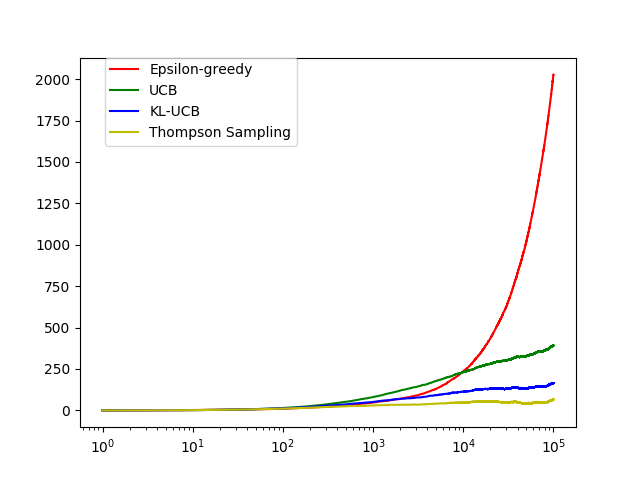
\includegraphics[scale=1]{images/Instance-5}
  \caption{Instance-5 All Algorithms}
  \label{fig:inst5_plot}
\end{figure}

\begin{figure}[H]
  \centering
  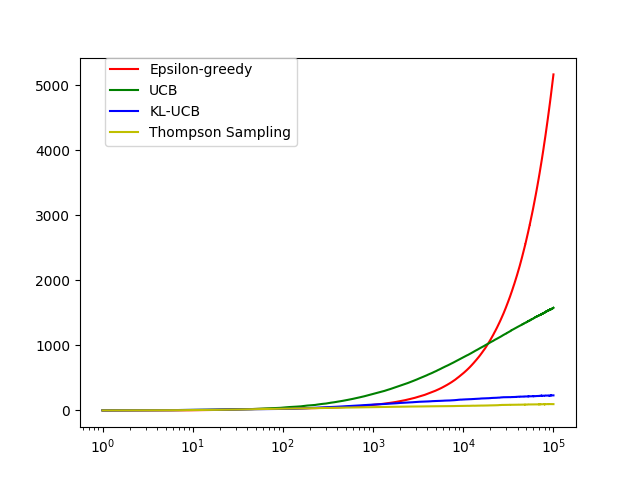
\includegraphics[scale=1]{images/Instance-25}
  \caption{Instance-25 All algorithms}
  \label{fig:inst25_plot}
\end{figure}

\section{Observations}
\subsection{Timing difference}
Interestingly there is quite some difference in the time taken by the algorithms for execution, and it is more apparent when the horizon is $100000$. In ascending order of time taken for completion of one run with horizon = $10^5$
$$\varepsilon - greedy < Thompson Sampling < UCB < KL-UCB$$.
Whereas in ascending order of regret it is (as can be seen from plots \ref{fig:inst5_plot}) and \ref{fig:inst25_plot})
$$Thompson Sampling < KL-UCB < UCB < \varepsilon - greedy$$
So it apparently seems Thompson Sampling does significantly better than the remaining algorithms.

\subsection{Log linear}
The plots in \ref{fig:inst5_plot} and \ref{fig:inst25_plot} clearly show that the Thompson Sampling, UCB and KL-UCB display linearly varying regret with respect to the log of the time instance. This is consistent with the theory taught in class. It is difficult to ascertain the relation of $\varepsilon - greedy$ but it does seem to be sub-polynomial in time (noting the linear plot in \ref{fig:inst5_lin})

\subsection{Negative Regret in some cases}
As noted earlier, the server side of the code is slightly modified to return the regret at each time instance. It was observed that for quite a few random seeds and at quite a few time instances the regret was shown to be negative. This is interesting because at first sight it seems that we are actually doing better than the best case possible. But it turns out that when averaged over all the runs the regret is positive [at any specific time instance], implying that the negative regret was mainly because of the stochastic nature of the server side.

\subsection{Choosing suboptimal arms at lower horizon}
It is noted that for each of the algorithms for instance-5 and horizon = $400$, the optimal arm is not always the one which is pulled maximum times. For example in the case of random seed 0, and horizon 400, the UCB algorithm pulled arm 3 (arm numbers indexed starting from 0) whose actual probability of success was 0.4 while the optimal arm was in fact arm 4 whose probability of success was $0.5$. It turns out that increasing the horizon to $10000$ and above solves this problem and the algorithm eventually starts choosing the optimal arm.

\subsection{Jittery graph for instance-5}
At first sight, the jittery graph seems a bit odd for instance-5, especially because it implies that regret could actually become less with more horizon, which is not true intuitively. In plotting the graph, 100 runs of each algorithm have been run, and regret at each instance is marked. So the only plausible explanation is that the decreased regret is only because of the stochastic nature of the experiment.

\subsection{Choosing the maximum}
This is less of an observation, more of an implementation detail. In dealing with ucb of individual arms, we have to break discrepancy when two arms have the same maximum value. In the code, the first occurence is always chosen. It is noted that making this deterministic doesn't really affect the regret on the average.

\subsection{Epsilon greedy doing better than UCB when horizon is small}
It is noted that for small horizons, Epsilon greedy approach (with $\varepsilon = 0.1$) actually outdoes UCB algorithm as can be seen in \ref{fig:inst5_lin}. The reason for this is presumably the reason that UCB algorithms pull the sub-optimal arms at smaller horizons and in general requires more time for exploration, whereas exploration in $\varepsilon - greedy$ is done stochastically and happens much faster. The problem that persists with $\varepsilon - greedy$ approach is that even after sufficient confidence about the optimal arm, it still tries to explore though it is exploration is not actually required. UCB circumvents this by creating the upper confidence bound, and restricts random explorations.
% [Plot linear plot]
\begin{figure}[H]
  \centering
  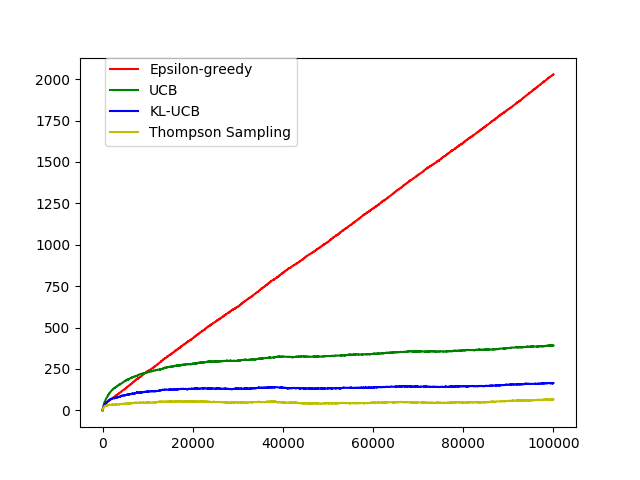
\includegraphics[scale=1]{images/Instance-5_linear}
  \caption{Linear Plot of Instance-5}
  \label{fig:inst5_lin}
\end{figure}

\section{Libraries used}
The client side is coded in python. The only modules used are {\bf Numpy} for random number generation, \textbf{socket} module for socket communication, \textbf{re} module to scrape the regret values, \textbf{Matplotlib} for graph plotting and \textbf{pdb} for debugging. The code has been run and tested on sl2 machine prior to submission.
\end{document}
